To understand what this paper about a few questions have to be answered first. What is a topological insulator? What is fractional topological insulator? What are dirac and weyl semimetals? What are quasiparticles? What do many body interactions change in these settings? In this section I will give the necessary background to understand both the questions we address and many of the techniques used to solve them. This will support the two papers this thesis is based upon~\cite{SahooSirotaGilTeo17}~\cite{RazaSirotaTeo17}.

\subsection{What is the quantum hall effect?}

To start, let's talk about the classical hall effect. For simplicity let's use a 2-D gas of electrons. First we need a material that when you apply an electric field, produces a current in a perpendicular direction. An important quality here is that such a current breaks time reversal symmetry. There are two directions the current could choose, and yet it only goes in one. An easy way to break this symmetry is by turning on a perpendicular magnetic field. If we just classically use the Lorentz Force to look for a steady state, we would find, and we assume $E=|E|\hat{x}$ and $B=|B|\hat{z}$
\begin{align}
F = -e(E+v \times B) = 0 \\
|E|\hat{x} + v \times |B| \hat{z} =0 \\
v = -|E|/|B| \hat{y}\\
j = -nev = ne|E|/|B| \hat{y}
\end{align}
where n is the density of the electrons. Now, $J= \sigma E$ where $\sigma$ is the conductance tensor, in this case a 2x2 tensor. Since the current is in the y direction and the electric field is in the x direction, this gives $\sigma_{xy}= ne/|B| $ and $\sigma_{xx}= 0 $. and if we assume the material is rotationally invariant, $\sigma_{yy}= 0 $ and $\sigma_{yx}= -ne/|B| $. The resistivity tensor is just the inverse of the conductance tensor.
\begin{align}
\sigma = 
\begin{pmatrix}
0 & ne/|B| \\
-ne/|B| & 0
\end{pmatrix} \quad 
\rho = 
\begin{pmatrix}
0 & |B|/(ne) \\
-|B|/(ne) & 0
\end{pmatrix}
\end{align}
Experimental results confirms this for low B fields, but gives us quite stunning effects in larger fields, as seen in figure \ref{fig:quantumhall}. This is not linear at all in B! We can rewrite our $\sigma_{xy}$ by defining the filling factor $\nu=nh/eB$ which gives $\sigma_{xy} = \nu e^2/h$. It appears that this $\nu$ is constant on these flat sections of the data, which we call quantum hall plateaus. 

\begin{figure}
	\centering
	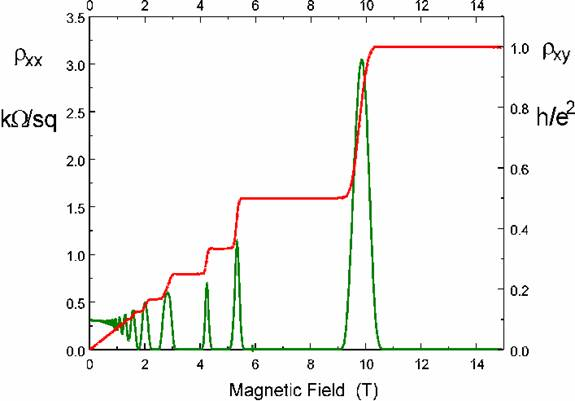
\includegraphics[width=0.5\linewidth]{images/QuantumHall}
	\caption{von Klitzing won the nobel prize in 1985 for discovering the quantum hall effect.}
		
		%from http://www.referatele.com/referate/fizica/online4/HALL-EFFECT---Explanation-of-the-Quantum-Hall-Effect-referatele-com.php$
	
	\label{fig:quantumhall}
\end{figure}

Now lets talk about laughlin's argument for this quantization.
Say we have a integer quantum hall state, like the graphene model. Put this on a cylinder of radius R with periodic boundary conditions. Let's use the coordinates x = x + R, and let y go from 0 to L. Then the allowed momentum around the cyclinder is quantized as $k_x= 2\pi n/R$ for n an integer. Then we will put a flux $\Phi$ through the cylinder as well a perpendicular B field, which we can do by having the vector potential $A(\theta,y) = (By+\Phi /R)\hat{x}$. Notice that the $By$ term gives us a magnetic field in the z direction, which makes this a 2-D gas of electrons in a magnetic field. The constant $\Phi/R$ just gives us that much more flux then we had previously. This gives us the Hamiltonian 
\begin{align}
H = \frac{p_y^2 +(p_x-eA)^2}{2m} = \frac{p_y^2 +(\hbar k_x - eA)^2}{2m} \\
= \frac{p_y^2}{2m} +\frac{(\hbar 2\pi n/R-eBy-e\Phi /R )^2}{2m}\\
= \frac{p_y^2}{2m} +\frac{(eB)^2}{2m}(y-\frac{hn}{eBR}+\frac{\Phi }{RB} )^2
\end{align}
Which you might recognize as the simple harmonic oscillator Hamiltonian, just with y shifted by $\frac{hn}{eBR}+\frac{\Phi }{RB}$ or $(n-\frac{e\Phi}{h})\frac{h}{eBR}$, with $\frac{1}{2}m\omega^2 = \frac{(eB)^2}{2m}$
Notice that if we shift $\Phi$ by $h/e$, that is the same as replacing n with n+1 in the Hamiltonian. This is what we call the flux quantum $\Phi_0$. So we have a series of states that are free in the x direction, and harmonic oscillators in the y direction, each one centered at some y that depends on the momentum in the x direction. If we add a flux quantum, that moves all the quantum states vertically by one spacing; it acts like an incompressible liquid. This essentially moves charge from one end of the cylinder to the other end. Since we have an integer number of filled harmonic oscillator states on each oscillator center, and the Hamiltonian goes back to itself after increases $\Phi$ by $\Phi_0$, we know we haved moved an integer number of electrons. Now $\Delta Q = I \Delta T = \sigma_{xy}E \Delta T = \sigma_{xy} \Delta \Phi = \sigma_{xy} h/e = \nu \frac{e^2h}{he} = \nu e $ . This argument shows that $\nu$ is an integer and explains the integer quantum hall effect! More important for this paper however if the fact that we can shrink one of the edges of the cylinder to a point. Then that is the point that the flux goes through. If we then pump charge to it, we will have an electron bound to the flux at a general point in a 2D material. This is a composite particle, since it is localized, and may have interesting properties.

\subsection{What is the fractional quantum hall effect?}

The extrapolation of this to the fractional quantum hall effect is actually quite simple. If you have states where $\nu$ is a fraction, then we can use the charge pump problem, and then between $\Phi$ and $\Phi + \Phi_0$, we get an identical hamiltonian, except a charge of $\nu e$ has been moved from one side to another. Since this has been done adiabatically, we know that this is an eigenstate. We have to accept that there exist local excitations that have a fractional amount of charge. Of course, these states are built out of electrons, and are just parts of a many-body electron wavefunctions. Again if we shrink part of the cylinder to a point, then the state is tied to a flux. Then we have a fully movable local quasiparticle with fractional charge and flux. Another important consequence is described through partice exchange. Normally if you exchange two fermions, you pick up a sign on the wavefunction, or a phase of $\pi$, and nothing if they are bosons. Here we have a fractional charge though, so there is no reason for that to hold. If we look at braiding, which is simply exchanging 2 particles twice, or topologically equivalent to having one particle make a circle around the other and return to it's original position, we can get an Aharonov Bohm phase. We call it braiding since the world line of these particles looks exactly like a braid. In 3 dimensions or higher, if you braid a particle around another, that is topologically equivalent to doing nothing, but in 2 dimensions, you in general have an integer number of classes of distinct topological paths, corresponding to how many times on particle wraps around the other, which is why you can get complex braiding phases. Particle statistics are in a sense, an action of the braid group on the wavefunction. Back to our case, if we have one stationary quasiparticle tied to a quantum of flux, and the move a particle of charge $e\nu$, then we will get a phase of $e\nu\Phi_0/\hbar$ or  $2\pi\nu$. That means the exchange phase has to be $\pi \nu$ which if $\nu$ is a fraction is completely new. You can define the topological spin $h$ in terms of these braiding phases, with $\theta_{a}=e^{2\pi i h}$, where $\theta_{a}$ is the exchange phase of a with a. You can see that a fermion has a -1 phase and bosons have a phase of 1. This is why we call these quasiparticles anyons, as opposed to fermions and bosons, since they can in principle have "any" spin. 

Laughlin described a trial wavefunction that approximates well the $\nu = 1/q$ ground state, which gives $> 99\%$ overlap with the numerically calculated ground state.

Laughlin's wave function is 
\begin{align}
\Psi(z_1,z_2,...,z_n) = \prod_{j<k}(z_j-z_k)^q \exp^{-\sum_i(|z_i|^2eB/4\hbar)}
\end{align} 
They guessed the form of this by assuming it would have a "Jastrow" form component $\prod_{j<k}f(z_j-z_k)$, which is translation invariant, and takes into account 2 body interactions. The exponential term  localizes each electron. Notice that q has to be odd in order for the wavefunction to be antisymmetric. He also described an operator which locally creates the excitation at $z_0$ with -1/q charge, or removes a flux quanta, which is just $\prod_{j<k}(z_j-z_0)$. You can use this to find out the braiding statistics, and use general quantum mechanics to find the charges. You can easily guess however that since an electron adds a  $\prod_{j<k}(z_j-z_0)^q$, along with an exponential suppression, that this operator is just 1/q of that. There is experimental evidence of these fractional charges, as well as these strange statistics. Haldane and later Halperin showed that if we have a Laughlin state, you can take some of the excitations, and create another Laughlin state out of those, much like the Laughlin state is made of electron operators, to get filling fractions of any odd denominator. These are called hierarchy states. 

A basic picture to understand what is happening here described by Jain is that $\nu = \frac{nh}{eB}$, but $\frac{h/e}{BA}$ where A is the area of the state, is one over the number of flux quantums, and n is the density of electrons. That means $\nu = \frac{nhA}{eBA} = \frac{nA}{\#\Phi_0} = \frac{\#elec}{\#\Phi_0}$. So the fraction really descibes a ratio between fraction of electrons to flux quanta. The idea to make a non interacting composite system is that eletrons don't interact with even amounts of fluxes, since they get $\pi$ phases around one but none with 2. If we want to recreate our original state out of just composite fermions and a magnetic field, we need the same filling fraction $\nu$, or $\nu$ electrons for each flux. So we'd need a density $\nu$ per flux of composites to get the charge, but we would then need a density of $2m\nu$ of fluxes on top of the external flux to cancel out the even number of fluxes attached to the composites. So then each composite sees a magnetic flux density of $2m\nu+1$, so we can create an integer quantum hall state with filling $p = \frac{\nu}{2m\nu+1}$ out of composites, which correspondes to an original state with a filling fraction for eletrons of $\nu = \frac{p}{2mp-1}$. We already know the integer quantum hall state is a non compressible non interacting liquid, so this works as a model for the fractional state. 

Another interesting fact about fractional quantum hall states is when you put them on a torus, you get degeneracy. If you introduce a flux and an antiflux at some point, they can go around one of the nontrivial torus loops and annihilate. Now we can label the 2 different ways you can do this by $T_1$ and $T_2$. You could think of acting with the operators in the following way $T_1^{-1}T_2^{-1}T_1T_2$, which is the commutator of these 2 operators. Now since after you act with a T operator, you are left behind with a flux line that loops around the torus, and we know that in general these fluxes can braid, which means their commutator is in general non-zero. Yet, these T operators certainly commute with the hamiltonian. This means if we start in a ground state that is also an eigenstate of $T_1$, $|\psi>$ and go to $T_2|\psi>=e^{i\theta}|\psi>$, that would mean the T's commute, but they don't so $T_2$ must bring the system to a distinct ground state, i.e. topological ground state degeneracy. In general the braiding phases we talked about ealier, don't just have just be a phase, but could change ground states, i.e. be a represented as a matrix on the space of ground states. This is known as a non abelian topological phase.

As an important aside in the section we saw the formulation of two very special things, quasiparticles with fractional charge and fractional statistics. Now if we wanted to classify fractional quantum hall states, we would have to start looking at either symmetries or topological invariants. If two states have topologically distinct quasiparticles, then they are definitely different phases, since the braiding rules can't change continuously. Even if we just restrict ourselves to the class without symmetry in just 2 dimensions, you could possibly create a hopeless number topologically distinct quasiparticles, thrown into an even larger size of different states. It turns out there are rules that govern what types of quasi-particles you can have, like locality and unitarity, that place this into the branch of mathematics called modular tensor category theory. Even then this is not a solved problem. This is very abstract still, since only a few of the many possible states allowed by modular tensor category theory have been experimentally realized, and many of those states can be well understood using the composite description above.

\subsection{The Pfaffian states}

So of interest in my work specifically is not an odd denominator state, but even. It would be useful to be able to have an operator that is like the square root of the electron creation operator. The reason being that for the Dirac semimetal paper~\cite{RazaSirotaTeo17}, we could write them in terms of $v=1/2$ operators, and then possibly interactions with these operators can gap the semimetal in a symmetric way. That would be inherently an highly interacting phases, and is precisely the solution we are looking for.

The Moore Read state~\cite{MooreRead,ReadMoore,GreiterWenWilczekPRL91,GreiterWenWilczek91} provides a possible description of a $v=5/2$ state. The first 2 landau levels are inert, so we will just look at the half filled third level. Notably these states we will talk about then have $v=1/2$ theoretically, even though there is no $v=1/2$ state experimentally. The 2 "inert" landau levels are actually vital to the states existence, but the results of this approximation seem to apply well to the $v=5/2$ state. Essentially you have the same composite fermion description, i.e. 2 fluxes for each electron. Now instead of making an integer quantum hall state with them, which would only yield odd denominator filling fractions, just like in superconducting theory, you combine them to make a "cooper pair" and then open up a "superconducting" gap. You can open this gap in a number of ways, which gives rises to many possible states. Since these are not actual electrons it does not mean the actual state is superconducting. In particular Moore and Read wrote down a trial wave function very similar to the Laughlin wavefunction.

In order to know how they got this wavefunction, you need to understand some conformal field theory, which will be useful later so we will give a brief overview here.

\subsubsection{Conformal Field Theory and Cherns Simons Theory Aside}
Conformal field theory evolved from string theory. It describes field theories that have a conformal symmetry, which is spatial/time transformation that leaves the metric $g_{\mu \nu}$ unchanged up to multiplying it by a constant. It turns out in 1+1 dimensions, at a critical point, if you have a local Lagrangian you will have conformal symmetry. Even for non critical theories fractional quantum hall theories, if they are Abelian they are described by a Cherns Simons theory. Witten showed the Chern Simons 2+1-d excitations correspond to primary fields on the edge. Abelian Cherns Simons Theories describe most of fractional quantum hall states, and there is powerful formalism for them. The ablelian Cherns Simons term is a gauge invariant term in 2+1 dimensions, 
\begin{align}
\mathcal{L}_{CS} = \frac{1}{4\pi}\varepsilon^{\mu \nu \lambda }K_{IJ}a_\mu^I\partial_\nu a^J_\lambda -e A_\mu t_I \partial_\nu a^I_\lambda \varepsilon^{\mu \nu \lambda }
\end{align}
Which corresponds to 1+1 d conformal field theory of 
\begin{align}
\mathcal{L}_{CFT} = \frac{1}{2\pi}\partial_t\phi^I K_{IJ} \partial_x\phi^J + ...
\end{align}

Where the NxN coupling matrix K is creatively called the "K matrix", $a$ and $\phi$ are N component U(1) gauge fields, A is the electromagnetic gauge field and the coupling t is a called the charge vector. K must be integer valued to be gauge invariant. Notice the low energy excitations of this theory are given by the potential energy, meaning not just any combinations of $\phi$'s are there. This matrix follows through to the conformal field theory, and together with the charge vector, you can use it to find out what all your excitations are in terms of your fields, their fusion rules and their braiding statistics. The K matrix defines an integer anyon lattice $\Gamma^*=\mathbb{Z}^N$, where a vector $b=(b_1,b_2,...b_N)$ corresponds to a creation operator of an anyon $\psi_b=e^{i b \cdot \phi}$ on the ground state. Fusion then is just vector addition in this lattice. The charge of this anyon is given by $q_a = t^TK^{-1}a$ Many of these particles are local bosons, specifically, any excitations given by $K\mathbb{Z}^N$ do not braid with anything, so we usually talk about just anyons in $\mathbb{Z}^N/K\mathbb{Z}^N$, which contains det|K| elements. The canonical commutation relations give you how creation and annihilation operators commute, which gives you the exchange phases and hence braiding. The braiding phase of anyons a around b is $\theta_{a,b} = e^{2\pi i a^T K^{-1} b}$, and the topological spin of a particle is defined by a 360 twist, or equivalently the phase it is exchanged with itself i.e. half a braiding phase. $\theta_a=\sqrt{\theta_{a,a}} = e^{\pi i a^T K^{-1} a} = e^{2 \pi i h_a}$ or $h_a = a^T K^{-1} a /2$ mod 1. You can check an exchange phase of -1 corresponds to spin 1/2. Notice also that braiding and fusion are related. If you do a 360 twist of particle c, and c = a x b, you are also braiding a around b, with a 360 twist of a and b. The $2\pi$ monodromy phase $\mathcal{M}^{XY}_Z=R^{XY}_ZR^{YX}_Z$ between primary fields $X$ and $Y$ with a fixed overall fusion channel $Z$ can be deduced by the {\em ribbon identity}~\cite{Kitaev06} \begin{align}e^{2\pi ih_Z}=\vcenter{\hbox{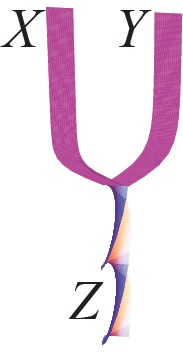
\includegraphics[width=0.5in]{ribbon1.jpg}}}=\vcenter{\hbox{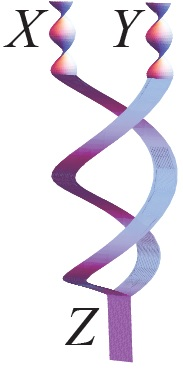
\includegraphics[width=0.5in]{ribbon2.jpg}}}=\mathcal{M}^{XY}_Ze^{2\pi i(h_X+h_Y)}\label{ribbonapp}\end{align} for $h_{X,Y,Z}$ the conformal spins for primary fields $X,Y,Z$. Unlike the gauge dependent $\pi$-exchange phase $R^{XY}_Z$, the $2\pi$-monodromy phase $\mathcal{M}^{XY}_Z=e^{2\pi i(h_Z-h_X-h_Y)}$ is gauge independent and physical. This means with just the spins and fusion rules you can derive the braiding statistics. Not only that but you can calculate $\sigma_{xy} = tK^{-1}t$ in units of the quantum conductance. You can check that all of this is consistent with the Laughlin theory having a K matrix of 3, and a charge vector of 1. We will use this quite often, so here is a summary of these important formulas.

\begin{align}
\theta_{a,b} = e^{2\pi i a^T K^{-1} b} \label{eq:transform1}\\
h_a = a^T K^{-1} a /2 \mod 1 \label{eq:transform2}\\
\theta_{a,b}= h_{a\times b}-h_a-h_b  \label{eq:transform3}\\
q_a = t^TK^{-1}a \label{eq:transform4}\\
\sigma_{xy} = t^TK^{-1}t \label{eq:transform5}
\end{align}

You can obviously do a change of basis, described by the following 
\begin{align}
\tilde{\phi}=M\phi \quad M^T\tilde{K}M=K \quad \tilde{t}=Mt
\end{align}


Notably, not all theories are abelian, although there is non abelian cherns simons theories, they are not so straightforward to describe. Now I will describe the general structure of conformal field theory.  For a more in depth introduction, see http://www.damtp.cam.ac.uk/ user/tong/string/four.pdf. 

In 2 dimensions, conformal field theory typically uses $z = t + ix$  and $\bar{z}= t - ix$ instead of using space and time coordinates, because conformal transformation then take the form $z \rightarrow f(z)$ and $\bar{z} \rightarrow \bar{f}(\bar{z})$. In this way we need can split the theory into just the z or $\bar{z}$ dependent pieces. We can look at infinitesimal forms of this or $z \rightarrow z + \epsilon(z)_n$ where $\epsilon(z)_n = -z^{n+1}$, which is generated by $l_n = -z^{n+1}\partial_z$. Notice that $l_0+\bar{l}_0$ and $i(l_0-\bar{l}_0)$ generate scaling and rotations. Notably in a quantum theory, our infinitesimal transformations can be generated using the stress energy tensor, and we may have some nontrivial commutation going on. In conformal theories, our stress energy tensor also breaks up into 2 parts, $T_{zz}(z)$ and $T_{\bar{z}\bar{z}}(\bar{z})$, with $T_{zz} =T_{\bar{z}\bar{z}}=0$. If we break our stress energy tensor into moments, $L_n$ they will follow similar commutation relations as $l_n$, except there is an extra piece called the central charge on the commutation of $L_n$ and $L_{-n}$. Their algebra is called the Virasoro algebra.

There is a notion of primary fields, which transform a specific way under a conformal transformations, $ \Psi(z,\bar{z}) \rightarrow (\frac{\partial f}{\partial z})^h (\frac{\partial \bar{f}}{\partial \bar{z}})^{\bar{h}}  \Psi(f(z),\bar{f}(\bar{z}))$, where $h$ and $\bar{h}$ are called the conformal weights. These are important to remember since they are eigenstates of scaling and rotations, so $h-\bar{h}$ is the spin and $h+\bar{h}$ is the eigenvalue of scaling. That makes them eigenstates of Virasoro operators $L_n$, or a representation of the algebra. This is a little different then field theory, where we call the functions we integrate the path integral over fields, here fields are just any function.

The next important piece is the operator product expansion. In general if we have a correlator of two local operators, $<O_1(z,\bar{z})O_2(w,\bar{w})>$, and we take a taylor expansion as w approaches z, we have the following definition of an operator product expansion
\begin{align}
<O_i(z,\bar{z})O_j(w,\bar{w})...> = \sum_k C^k_{ij}(z-w,\bar{z}- \bar{w}) O_k(w,\bar{w}...)
\end{align}
Where the sum is over all local operators. The ... part refers to the idea that this holds when these are followed by a string of other operators, as long as they are not close to z or w relative to the distance between them. The form of these C functions are restricted since we have conformal symmetry, for example must only depend on position differences due to translation symmetry. For example we could ask about our local excitations in the quantum hall effect as our local operators, then their operator product expansion would give us information about their fusion rules, i.e. what other local operators they're sum is described by. Something familiar are the clebsh gordon coefficients. This looks much like an algebra, but because of it's z dependence is given the name vertex algebra. It actually contains more information then fusion rules. If the operators are primary they are restricted to only have 2 divergent parts, with one proportional to the conformal weight. You can use the OPE to define primary as well.

If we find the operator product expansion of the stress energy tensor with itself, which is notably not primary, we get not just a weight term, but a $1/(z-w)^4$ term proportional to what's called the central charge. This piece's local operator is just the identity, so it adds some zero energy to your theory, also known as a Casimir energy. There is a theorem that says that the central change counts your degrees of freedom, and is related to the total heat current. For example $c=\bar{c}=n$ for n scalar fields (bosons), and $c=\bar{c}=n/2$ for n free fermion fields.

Finally we have the idea of rational conformal field theories, which is where you can get all of the possible fields from a finite number of primary fields, which are representations of the virasoro algebra, and then by acting on them with "lowering" operators, that change their conformal weights. These are nice since they are completely solvable given just symmetry arguments. A good analogy here are the spin states, where given a highest spin you can have all the possible types by acting with lowering operators, and then at some point the sequence will terminate.

Moore and Read found a way to write the laughlin wavefuntion as a correlator of fields. Then they used that same prescription to find a wave function for a $\nu=1/2$. The real wavefunction would be this on top of the wavefunction of 2 completely filled landau levels. 
\begin{align}
\Psi(z_1,z_2,...,z_n) = Pf(\frac{1}{z_i-z_j})\prod_{j<k}(z_j-z_k)^2 \exp^{-\sum_i(|z_i|^2eB/4\hbar)}
\end{align}

Where $Pf$ is the pfaffian of a skew-symmetric matrix. It is defined as a polynomial in the matrix entries with integer valued coefficients such that $Pf(M)^2=det(M)$.  The term falls out of wicks theorem when you apply it to real fermion fields. The important thing about this term is that it lets the wavefunction be antisymmetric, when q = 2. Using this ground state, you can find what the elementary excitations are. Since the electrons or composite fermions are paired, when you braid them around a flux you get twice the phase. This means the flux quantum is halved. So now when you go through the charge pump argument the elementary excitation has charge $\nu e/2 = e/4$, modulo e. When we analyze the braiding statistics of this particle with our electron, we get a phase of 1, and when we look at it's spin $h$, which we define by the phase of braiding it around another copy of itself, $e^{2\pi i h}$, we get $h=1/16$. This primary field also ends up being non-abelian, i.e. it's OPE with itself gives a two primary fields, a fermion and a boson with charge e/2. In this way all the excitations are produced. This Moore-Read state can be described as a decomposition into $Ising \otimes U(1)_4$ Where the $U(1)_4$ is just particles of charge $ne/4$, where n is an integer from 0 to 7, called $e_1,e_2,...e_7$, and the Ising theory is the majorana fermion $\psi$, and the $\pi$ flux $\sigma$, where we then remove anything that is not local with respect to the fermion. The excitations topological spins are described in Table ~\ref{tab:Pfaff}.
\begin{table}[h]
	\centering
	\begin{tabular}{|c|c|c|c|c|c|c|c|c|}
		\hline
		&$e_0$& $e_1$ & $e_2$ & $e_3$ & $e_4$& $e_5$& $e_6$& $e_7$\\
		\hline
		$\openone$ & 0 && 1/4 & & 0 && 3/4 & \\
		\hline
		$\sigma $ && 1/8 && 5/8 && 5/8 && 1/8 \\
		\hline
		$\psi$ & 1/2 && 3/4 & & 1/2 && 1/4 &\\
		\hline
		charge & 0 &e/4& 2e/4 & 3e/4 & e & 5e/4& 6e/4 & 7e/4\\
		\hline
	\end{tabular}
	\label{tab:Pfaff}
\end{table}

It is important to clarify and disambiguate the three "Pfaffian" fractional quantum Hall states that commonly appear in the literature. All these $(2+1)$D states are theorized at filling fraction $\nu=1/2$, although being applied to $\nu=5/2$ in materials, and have identical electric transport properties. However, they have distinct thermal Hall transport behaviors. They all have very similar anyonic quasiparticle structures. For instance, they all have four Abelian and two non-Abelian quasiparticles (up to the electron). On the other hand, the charge $e/4$ non-Abelian Ising anyons of the three states have different spin-exchange statistics. First, the gapless boundary of the Moore-Read Pfaffian fractional quantum hall state can be described by the $(1+1)$D chiral conformal field theory $U(1)_4\otimes\mathrm{Ising}$ where the charged boson and neutral fermion sectors are co-propagating. It therefore carries the chiral central charge $c=1+1/2=3/2$, which dictates the thermal Hall response \eqref{conductance}. Second, the ``anti-Pfaffian" fractional quantum hall state~\cite{LevinHalperinRosenow07,LeeRyuNayakFisher07} is the particle-hole conjugate of the Moore-Read Pfaffian state. Instead of half-filling the lowest Landau level by electrons, one can begin with the completely filled lowest Landau level, and half-fill it with holes. In a sense the anti-Pfaffian state is obtained by subtracting the completely filled lowest Landau level by a Moore-Read Pfaffian state. Along the boundary, the $(1+1)$D conformal field theory $U(1)_{1/2}\otimes\overline{U(1)_4\otimes\mathrm{Ising}}$ consists of the forward propagating chiral Dirac $U(1)_{1/2}$ sector that corresponds to the lowest Landau level, and the backward propagating Moore-Read Pfaffian $\overline{U(1)_4\otimes\mathrm{Ising}}$. Here $\overline{\mathcal{C}}$ can be interpreted as the time-reversal conjugate of the chiral conformal field theory $\mathcal{C}$. The thermal transport is governed by the edge chiral central charge $c=1-3/2=-1/2$, which has an opposite sign from the filling fraction. Thus, unlike the Moore-Read Pfaffian state, the net electric and thermal currents now travel in opposite directions along the edge. Lastly, the recently proposed particle-hole symmetric Pfaffian state~\cite{Son15,BarkeshliMulliganFisher15,WangSenthil16}, which is going to be the {\em only} Pfaffian fractional quantum hall state considered in this article (see Ref.~\onlinecite{KaneSternHalperin17} for a coupled wire construction), has the chiral edge conformal field theory \eqref{PfaffianCFT}. As the electrically charged boson and neutral fermion sectors are counter-propagating, the net thermal edge transport is governed by the chiral central charge $c=1-1/2=1/2$. The chiral $(1+1)$D particle hole symmetric Pfaffian conformal field theory \eqref{PfaffianCFT} is also present along the line interface separating a time reversal symmetric $\mathcal{T}$-Pfaffian~\cite{ChenFidkowskiVishwanath14} domain and a time reversal breaking magnetic domain on the surface of a 3D topological insulator. (Similar constructions can be applied to alternative time reversal symmetric topological insulator surface states~\cite{WangPotterSenthilgapTI13,MetlitskiKaneFisher13b,BondersonNayakQi13}, but they will not be considered in this article.) Other than their thermal transport properties, the three Pfaffian fractional quantum hall state can also be distinguished by the charge $e/4$ Ising anyon, which has spin $h=1/8$, $-1/8$ or $0$ for the Moore-Read Pfaffian, anti-Pfaffian or particle hole symmetry Pfaffian states respectively. 

Since we will not be considering the Moore-Read Pfaffian or its particle-hole conjugate anti-Pfaffian state, we will simply refer to the particle hole symmetry Pfaffian state as the Pfaffian state. It's actually true that there are other abelian theories that describe a $\nu=1/2$ state, but we do not work with them here.

\subsection{Pfaffian Field Theory}
Now the piece de resistance, the reason why we focus on this Pfaffian state is the fact that many-body interactions can facilitate the fractionalization of a $(1+1)$D chiral Dirac channel \begin{align}\mathrm{Dirac}=\mathrm{Pfaffian}\otimes\mathrm{Pfaffian}\label{fractionalization}\end{align} (see also figure~\ref{fig:glueingsplitting}). In a sense, each chiral Pfaffian channel carries half of the degrees of freedom of the Dirac. For instance, it has half the electric and thermal conductances, which are characterized by the filling fraction $\nu=1/2$ and the chiral central charge $c=1/2$ in \eqref{conductance}. Through out this paper, we refer to the low-energy effective  -- that consists of an electrically charged $U(1)_4$ bosonic component,conformal field theory say moving in the $R$ direction, and a neutral Majorana fermion component moving in the opposite $L$ direction -- simply as a Pfaffian conformal field theory \begin{align}\mathrm{Pfaffian}=U(1)_4\otimes\overline{\mathrm{Ising}}.\label{PfaffianCFT}\end{align} (In this article, we follow the level convention for $U(1)$ in the conformal field theory community~\cite{bigyellowbook}. The same theory may be more commonly referred to as $U(1)_8$ in the fractional quantum Hall community. For clarification, see Lagrangian \eqref{Pfaffian} and \eqref{LFQHCS}.)

The low-energy effective chiral $(1+1)$D conformal field theory takes the decoupled form between the boson and fermion \begin{align}\mathcal{L}_{\mathrm{Pfaffian}}&=\mathcal{L}_{\mathrm{charged}}+\mathcal{L}_{\mathrm{neutral}}\label{Pfaffian}\\&=\frac{8}{2\pi}\partial_t\phi_R\partial_x\phi_R+v(\partial_x\phi_R)^2\nonumber\\&\;\;\;+i\gamma_L(\partial_t-\tilde{v}\partial_x)\gamma_L\nonumber\end{align} where we have set $\hbar=1$. Here $\phi_R$ is the free chiral $U(1)_4$ boson. It generates the $(1+1)$D theory $\mathcal{L}_{\mathrm{charged}}$, which is identical to the boundary edge theory of the $(2+1)$D bosonic Laughlin $\nu=1/8$ fractional quantum Hall state described by the topological Chern-Simon theory~\cite{WenZee92,Wenedgereview} \begin{align}\mathcal{L}_{2+1}=\frac{K}{4\pi}\alpha\wedge d\alpha+et\alpha\wedge dA\label{LFQHCS}\end{align} with $K=8$ and $t=2$. The $U(1)_4$ conformal field theory carries the electric conductance $\sigma=tK^{-1}t=1/2$ in units of $2\pi e^2=e^2/h$ and a thermal conductance characterized by the chiral central charge $c=c_R=1$. Primary fields are of the form of (normal ordered) chiral vertex operators $:e^{im\phi_R}:$, for $m$ an integer, and carries charge $q=m/4$ in units of $e$ and conformal scaling dimension (i.e.~conformal spin) $h=h_R=m^2/16$. We summarize and abbreviate the operator product expansion \begin{align}e^{im_1\phi_R(z)}e^{im_2\phi_R(w)}=e^{i(m_1+m_2)\phi_R(w)}(z-w)^{m_1m_2/8}+\ldots\end{align} by the Abelian fusion rule \begin{align}e^{im_1\phi_R}\times e^{im_2\phi_R}=e^{i(m_1+m_2)\phi_R},\end{align} where $z\sim\tau+ix$ is the complex space-time parameter and $\tau=i\pi vt/2$ is the Euclidean time.

$\gamma_L^\dagger=\gamma_L$ is the free Majorana fermion. It generates the $(1+1)$D theory $\mathcal{L}_{\mathrm{neutral}}$, which is equivalent to a chiral component of the critical Ising conformal field theory or the boundary edge theory of the $(2+1)$D Kitaev honeycomb model~\cite{Kitaev06} in its B-phase with time reversal breaking (i.e.~a chiral $p_x+ip_y$ superconductor coupled with a $\mathbb{Z}_2$ gauge theory). It carries trivial electric conductance but contributes to a finite thermal conductance characterized by the chiral central charge $c=-c_L=-1/2$. The Ising conformal field theory has primary fields $1$, $\gamma_L$ and $\sigma_L$, where the twist field (or Ising anyon) $\sigma_L$ carries the conformal spin $h=-h_L=-1/16$. Again, we abbreviate the operator product expansions \begin{gather}\gamma_L(\bar{z})\gamma_L(\bar{w})=\frac{1}{\bar{z}-\bar{w}}+\ldots\nonumber\\\sigma_L(\bar{z})\gamma_L(\bar{w})=\frac{\sigma_L(\bar{w})}{(\bar{z}-\bar{w})^{1/2}}+\ldots\nonumber\\\sigma_L(\bar{z})\sigma_L(\bar{w})=\frac{1}{(\bar{z}-\bar{w})^{1/8}}+(\bar{z}-\bar{w})^{3/8}\gamma_L(\bar{w})\nonumber\end{gather} by the fusion rule \begin{gather}\gamma_L\times\gamma_L=1,\quad\sigma_L\times\gamma_L=\sigma_L\nonumber\\\sigma_L\times\sigma_L=1+\gamma_L,\end{gather} where $\bar{z}\sim\tau-ix$ is the complex space-time parameter and $\tau=i\tilde{v}t$ is the Euclidean time. 

General primary fields of the Pfaffian conformal field theory decompose into the $U(1)_4$ part and the Ising part. They take the form \begin{align}1_m=e^{im\phi_R},\quad\psi_m=e^{im\phi_R}\gamma_L,\quad\sigma_m=e^{im\phi_R}\sigma_L.\label{Pfaffianfields}\end{align} The conformal spins and fusion rules also decompose so that \begin{align}h_{1_m}=\frac{m^2}{16},\quad h_{\psi_m}=\frac{m^2}{16}+\frac{1}{2},\quad h_{\sigma_m}=\frac{m^2-1}{16}\end{align} modulo 1, $q_m=m/4$ in units of $e$, and \begin{gather}1_{m_1}\times1_{m_2}=\psi_{m_1}\times\psi_{m_2}=1_{m_1+m_2}\nonumber\\1_{m_1}\times\psi_{m_2}=\psi_{m_1+m_2}\nonumber\\1_{m_1}\times\sigma_{m_2}=\psi_{m_1}\times\sigma_{m_2}=\sigma_{m_1+m_2}\nonumber\\\sigma_{m_1}\times\sigma_{m_2}=1_{m_1+m_2}+\psi_{m_1+m_2}.\end{gather} 

The electronic quasiparticle is the composition $\psi_{\mathrm{el}}=e^{-i4\phi_R}\gamma_L$ so that it is fermionic and has electric charge $-1$ in units of $e$. Since electron is the fundamental building block of the system, locality of $\psi_{\mathrm{el}}$ only allows primary fields $X$ that have trivial monodromy $\mathcal{M}^{X,\psi_{\mathrm{el}}}=1$ with the electron. As a result, this restricts $1_m,\psi_m$ to even $m$ and $\sigma_m$ to odd $m$. Lastly, the coupled wire models constructed later will involve the Pfaffian channels that propagate in both forward and backward directions. We will denote the backward case by $\overline{\mathrm{Pfaffian}}$, whose Lagrangian density is the time reversal of \eqref{Pfaffian}, i.e.~replacing $R\leftrightarrow L$, $i\leftrightarrow-i$ and $\partial_t\leftrightarrow-\partial_t$. 

\subsubsection{Gluing and splitting}\label{sec:gluing}

\begin{figure}[htbp]
	\centering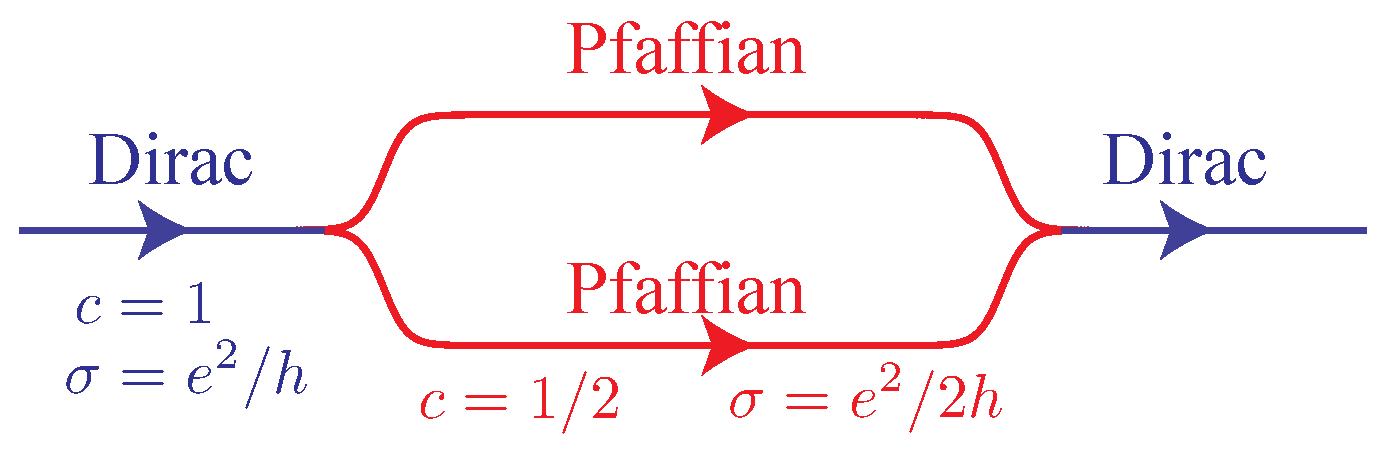
\includegraphics[width=0.3\textwidth]{glueingsplitting}
	\caption{Gluing and splitting a pair of chiral Pfaffian 1D channels into and from a chiral Dirac channel.}\label{fig:glueingsplitting}
\end{figure}

A pair of co-propagating Pfaffian conformal field theory can be ``glued" together into a single chiral Dirac electronic channel. We first consider the decoupled pair $\mathcal{L}_0=\mathcal{L}_{\mathrm{Pfaffian}}^A+\mathcal{L}_{\mathrm{Pfaffian}}^B$, where $\mathcal{L}_{\mathrm{Pfaffian}}^{A/B}$ is the Lagrangian density of one of the two Pfaffian conformal field theory labeled by $A,B$. The pair of Majorana fermions can compose an electrically neutral Dirac fermion $d_L=(\gamma^A_L+i\gamma^B_L)/\sqrt{2}$, which can then be bosonized $d_L\sim e^{i\phi^\sigma_L}$, for $\phi^\sigma_L$ the chiral $\overline{U(1)_{1/2}}$ boson. Bosonization can be thought of as writing a fermion in terms of a boson, which usually ends up with the form $\psi\sim e^{i\phi}$, and you can rewrite the Lagrangian with this identity, although you cannot simply plug this in because you must be careful about normal ordering. For more detail see ~\cite{senechal99} The bare Lagrangian now becomes the multi-component $U(1)_4^A\otimes U(1)_4^B\otimes\overline{U(1)_{1/2}}$ boson conformal field theory \begin{align}\mathcal{L}_0=\frac{1}{2\pi}\partial_t\boldsymbol{\phi}^TK\partial_x\boldsymbol{\phi}+\partial_x\boldsymbol{\phi}^TV\partial_x\boldsymbol{\phi},\label{881}\end{align} where $\boldsymbol{\phi}=(\phi_R^A,\phi_R^B,\phi^\sigma_L)$, $K$ is the $3\times3$ diagonal matrix $K=\mathrm{diag}(8,8,-1)$, and $V$ is some non-universal velocity matrix. A primary field is a vertex operator $e^{i{\bf m}\cdot\boldsymbol{\phi}}$ labeled by an integral vector ${\bf m}=(m^A,m^B,\tilde{m})$. It carries conformal spin $h_{\bf m}={\bf m}^TK^{-1}{\bf m}/2$ and electric charge $q_{\bf m}={\bf t}^TK^{-1}{\bf m}$ in units of $e$, where ${\bf t}=(2,2,0)$ is the charge vector. We can use the Haldane criterion to find backscattering terms that gap out excitations~\cite{Haldane95}. The algorithm for finding them is to find null vectors, i.e.~${\bf n}^TK{\bf n}=0$.  As ${\bf n}=(1,-1,4)$ is an electrically neutral null vector (${\bf t}\cdot{\bf n}=0$), it corresponds to the charge $U(1)$ preserving backscattering coupling \begin{align}\delta\mathcal{H}=-u\cos\left({\bf n}^TK\boldsymbol{\phi}\right)=-u\cos\left(8\phi^A_R-8\phi^B_R-4\phi^\sigma_L\right)\label{glueingH}\end{align} that gaps and annihilates a pair of counter-propagating boson modes. The interacting Hamiltonian can also be expressed in terms of many-body backscattering of the Pfaffians' primary fields \begin{align}\delta\mathcal{H}=-u:\left(d_L^\dagger d_R\right)^4:+h.c.\end{align} where $d_R=1_2^A1_{-2}^B$ is the electrically neutral Dirac fermion composed of the pair of oppositely charged semions in the two Pfaffian sectors.

In strong coupling, the gapping Hamiltonian introduces an interacting mass and the ground state expectation value $\langle\Phi\rangle=n\pi/2$, for $n$ an integer and $\Phi=2\phi^A_R-2\phi^B_R-\phi^\sigma_L$. In low energy, it leaves behind the chiral boson combination $\tilde\phi_R=2\phi_R^A+2\phi_R^B$, which has trivial operator product (i.e.~commutes at equal time) with the order parameter $\Phi$. The low-energy theory after projecting out the gapped sectors becomes \begin{align}\mathcal{L}_0-\delta\mathcal{H}\longrightarrow\mathcal{L}_{\mathrm{Dirac}}=\frac{1}{2\pi}\partial_t\tilde\phi_R\partial_x\tilde\phi_R+v(\partial_x\tilde\phi_R)^2\end{align} which is identical to the bosonized Lagrangian density of a chiral Dirac fermion. For instance, the vertex operator $\psi_R^{\mathrm{el}}\sim e^{i\tilde\phi_R}\sim 1_2^A1_2^B$ has the appropriate spin and electric charge of an electronic Dirac fermion operator ($h=1/2$ and $q=1$ in units of $e$). Notice that the vertex operator $e^{i\tilde\phi_R/2}$ has $-1$ monodromy with the local electronic $\psi_R^{\mathrm{el}}$ and therefore is not an allowed excitation in the fermionic theory.

We notice in passing that the gluing potential \eqref{glueingH} facilitates an anyon condensation process~\cite{BaisSlingerlandCondensation}, where the maximal set of mutually local neutral bosonic anyon pairs \begin{align}\begin{array}{*{20}c}1_{4m}^A1_{-4m}^B,\psi_{4m}^A\psi_{-4m}^B,\\\psi_{4m+2}^A1_{-4m-2}^B,1_{4m+2}^A\psi_{-4m-2}^B,\sigma_{4m+1}^A\sigma_{-4m-1}^B\end{array}\label{condensebosons}\end{align} is condensed, where $m$ is an arbitrary integer. All primary fields that are non-local (i.e.~with non-trivial monodromy) with any of the condensed bosons in \eqref{condensebosons} are confined. Any two primary fields that differ from each other by a condensed boson in \eqref{condensebosons} are now equivalent. The condensation therefore leaves behind the electronic Dirac fermion \begin{align}\psi^{\mathrm{el}}_R=\psi^A_4\equiv\psi^B_4\equiv1_2^A1_2^B\end{align} and its combinations. 

\begin{figure}[htbp]
	\centering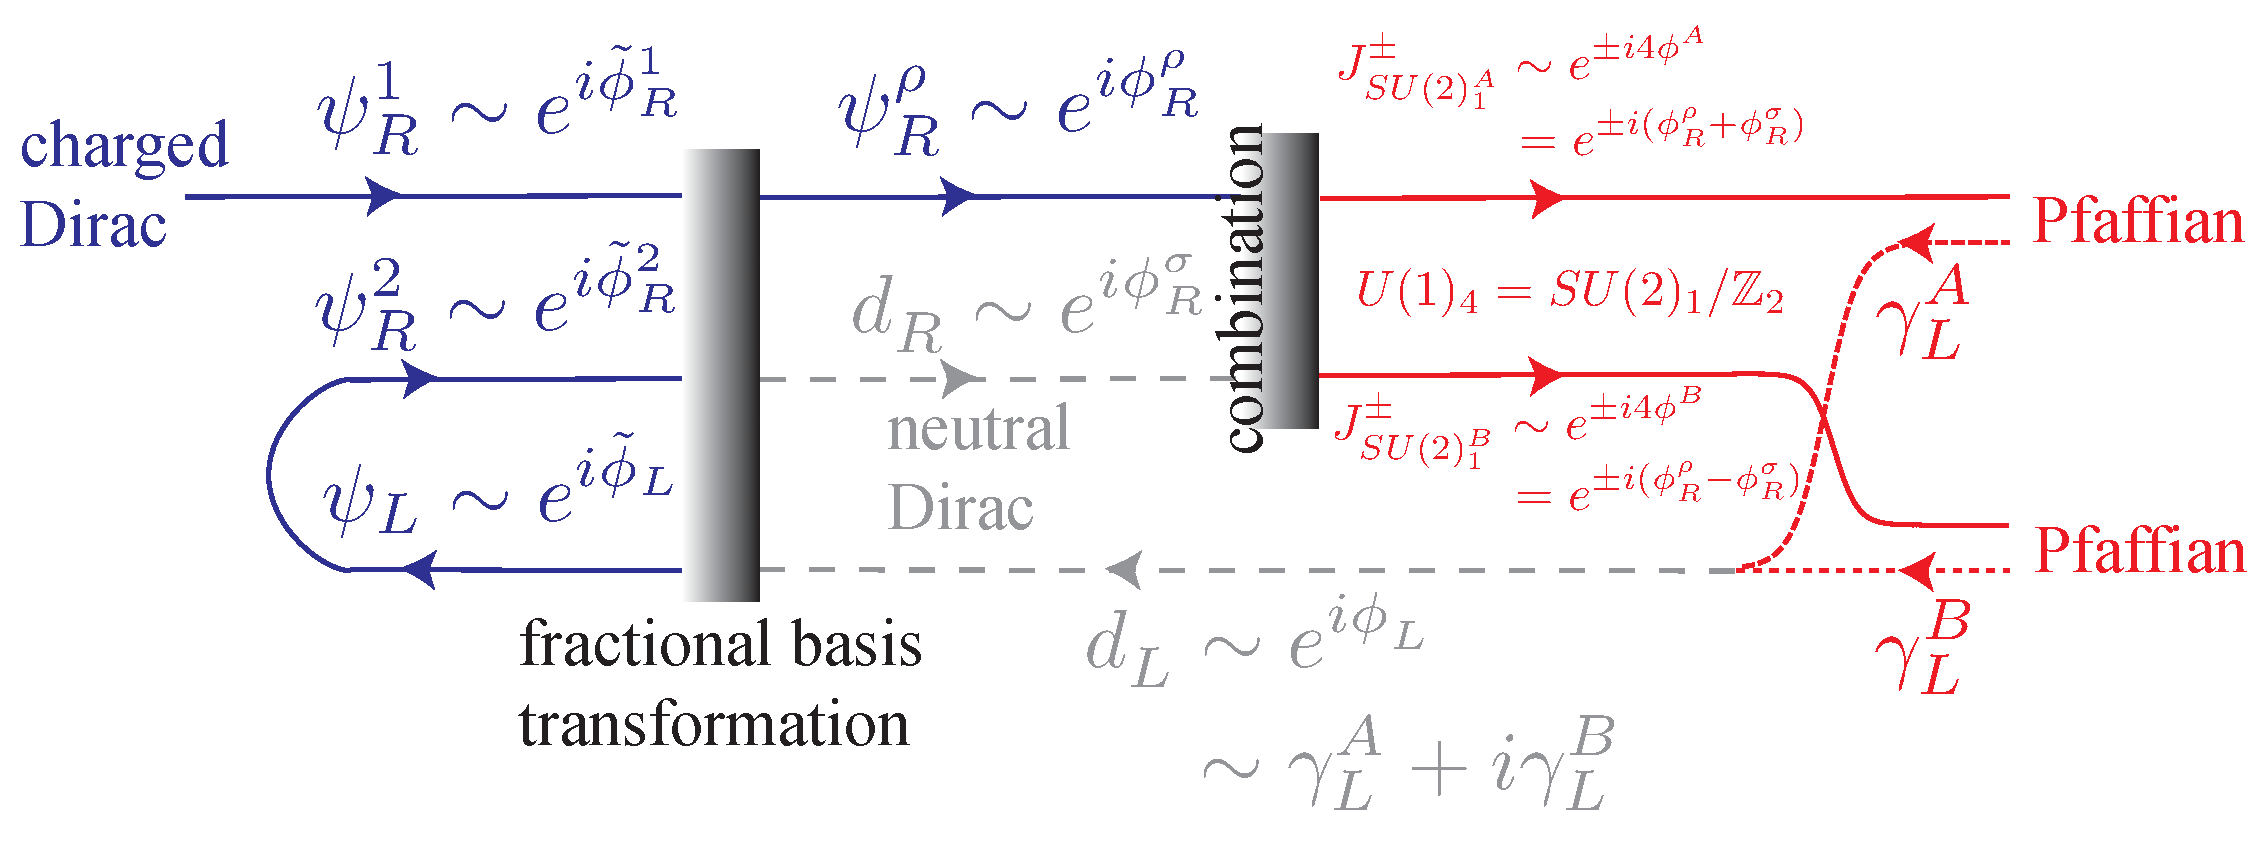
\includegraphics[width=0.5\textwidth]{fractionalization}
	\caption{Schematics of splitting a chiral Dirac channel into a pair of Pfaffian channels.}\label{fig:fractionalization}
\end{figure}

On the other hand, a chiral Dirac channel can be decomposed into a pair of chiral Pfaffian channels (see figure~\ref{fig:fractionalization} for a summary). The first problem is that the Pfaffian has many more degrees of freedom then a Dirac fermion. Perhaps from some channel re-construction, we append to the chiral Dirac channel an additional pair of counter-propagating Dirac modes. This can be realized by pulling a parabolic electronic/hole band from the conduction/valence band to the Fermi level, or introducing non-linear dispersion to the original chiral channel. In low-energy, the three Dirac fermion modes can be bosonized $\psi^{1,2}_R\sim e^{i\tilde\phi_R^{1,2}}$, $\psi_L\sim e^{-i\tilde\phi_L}$ and they are described by the multicomponent boson Lagrangian \begin{align}\widetilde{\mathcal{L}}_{\mathrm{Dirac}}=\frac{1}{2\pi}\partial_t\widetilde{\boldsymbol\phi}^T\tilde{K}\partial_x\widetilde{\boldsymbol\phi}+\partial_x\widetilde{\boldsymbol\phi}^T\tilde{V}\partial_x\widetilde{\boldsymbol\phi}\label{3Dirac}\end{align} for $\widetilde{\boldsymbol\phi}=(\tilde\phi_R^1,\tilde\phi_R^2,\tilde\phi_L)$, $\tilde{K}$ is the diagonal matrix $\tilde{K}=\mathrm{diag}(1,1,-1)$, and $\tilde{V}$ is some non-universal velocity matrix. A general composite excitation can be expressed by a vertex operator $e^{i{\bf m}\cdot\widetilde{\boldsymbol\phi}}$, for ${\bf m}$ an integral 3-vector, with spin $h_{\bf m}=|{\bf m}|^2/2$ and electric charge $q_{\bf m}={\bf m}^T\tilde{K}\tilde{\bf t}$ in units of $e$, where $\tilde{\bf t}=(1,1,1)$ is the charge vector.

Next we perform a {\em fractional} basis transformation \begin{align}\begin{array}{*{20}l}\phi^\rho_R=\tilde\phi^1_R+\tilde\phi^2_R+\tilde\phi_L\\\phi^\sigma_R=\tilde\phi^1_R-\frac{1}{2}\tilde\phi^2_R+\frac{1}{2}\tilde\phi_L\\\phi^\sigma_L=\tilde\phi^1_R+\frac{1}{2}\tilde\phi^2_R+\frac{3}{2}\tilde\phi_L\end{array}.\label{fracbasistrans0}\end{align} This follows the transformation rules from equations ~\ref{eq:transform1}~--~\ref{eq:transform5}. While the $\tilde{K}$ matrix is invariant under the transformation, the charge vector changes to $\tilde{\bf t}\to(1,0,0)$. $\psi^\rho_R\sim e^{i\phi^\rho_R}$ is the local electronic Dirac fermion that carries spin $1/2$ and electric charge $e$, and $d_{R/L}\sim e^{i\phi^\sigma_{R/L}}$ are counter-propagating electrically neutral Dirac fermions. As the $\tilde{K}$ matrix is still diagonal, these fermions have trivial mutual $2\pi$-monodromy and are local with respect to each other. However, it is important to notice that the neutral Dirac fermions $d_{R/L}$ actually consist of fractional electronic components.

Now we focus on the two $R$-moving Dirac channels. By pairing the Dirac fermions, they form two independent $SU(2)_1$ Kac-Moody current operators~\cite{bigyellowbook}. This is defined by the OPE in equation~\ref{SU2algebra}. \begin{align}J_3^{A/B}(z)&=i2\sqrt{2}\partial_z\phi^{A/B}_R(z)\label{SU2current}\\J_\pm^{A/B}(z)&=\frac{J_1^{A/B}(z)\pm iJ_2^{A/B}(z)}{\sqrt{2}}=e^{\pm i4\phi^{A/B}_R(z)}\nonumber\end{align} where $4\phi^A_R=\phi^\rho_R+\phi^\sigma_R$ and $4\phi^B_R=\phi^\rho_R-\phi^\sigma_R$. Both $SU(2)_1$ sectors are electrically charged so that the bosonic vertex operators $J_\pm^{A/B}$ carries charge $\pm e$. They obey the $SU(2)$ current algebra at level 1 \begin{align}J^\lambda_{\mathsf{i}}(z)J^{\lambda'}_{\mathsf{j}}(w)=\frac{\delta^{\lambda\lambda'}\delta_{\mathsf{ij}}}{(z-w)^2}+\sum_{\mathsf{k}=1}^3\frac{i\sqrt{2}\delta^{\lambda\lambda'}\varepsilon_{\mathsf{ijk}}}{z-w}J^\lambda_{\mathsf{k}}(w)+\ldots\label{SU2algebra}\end{align} for $\lambda,\lambda'=A,B$. It is crucial to remember that $J_\pm^A\sim\psi^\rho_Rd_R$ and $J_\pm^B\sim\psi^\rho_Rd_R^\dagger$ contains the fractional Dirac components $d_R$. Thus, the primitive local bosons are actually pairs of the current operators, i.e.~$e^{i8\phi^{A/B}_R}$. Equivalently, this renormalizes the compactification radius of the boson $4\phi^{A/B}_R$ so that in a closed periodic space-time geometry, we only require electronic Cooper pair combinations such as the charge $2e$ local operators \begin{gather}e^{i8\phi^A_R}=e^{i(4\tilde\phi^1_R+\tilde\phi^2_R+3\tilde\phi_L)}\sim(\psi^1_R)^4\psi^2_R(\psi_L^\dagger)^3\nonumber\\e^{i8\phi^B_R}=e^{i(3\tilde\phi^2_R+\tilde\phi_L)}\sim(\psi^2_R)^3\psi_L^\dagger\end{gather} to be periodic. The incorporation of anti-periodic boundary condition for $J_\pm^{A/B}=e^{\pm i4\phi^{A/B}_R}$ results in the $\mathbb{Z}_2$-orbifold theory~\cite{Ginsparg88,DijkgraafVafaVerlindeVerlinde99} $U(1)_4=SU(2)_1/\mathbb{Z}_2$ for both $A$ and $B$ sectors. Orbifolding usually results in new "twist" fields", or fields that when braided with the object that is can have antiperiodic boundary conditions, yeilds the -1 required. For instance, the primitive twist fields are given by $e^{\pm i\phi^{A/B}_R}$, which have $-1$ monodromy phase with $J_\pm^{A/B}$. 

At this point, including the $L$-moving neutral Dirac sector, we have recovered the muticomponent boson $\boldsymbol\phi=(\phi^A_R,\phi^B_R,\phi^\sigma_L)$ described by the Lagrangian \eqref{881}. Lastly, we simply have to decompose the remaining neutral Dirac into Majorana components, $d_L=(\gamma^A_L+i\gamma^B_L)/\sqrt{2}$. The $A$ and $B$ Pfaffian sectors can then be independently generated by the charged $U(1)_4$ boson $\phi^{A/B}_R$ and the neutral Majorana fermion $\gamma^{A/B}_L$. As a consistency check, the charge $e$ fermionic (normal ordered) combinations defined in \eqref{Pfaffianfields} \begin{align}\psi_4^A&\sim e^{i4\phi^A_R}\gamma_L^A\sim e^{i\tilde\phi^1_R}+e^{i(3\tilde\phi^1_R+\tilde\phi^2_R+3\tilde\phi_L)}\label{psi4def1}\\\psi_4^B&\sim e^{i4\phi^B_R}\gamma_L^B\sim e^{i(-\tilde\phi^1_R+\tilde\phi^2_R-\tilde\phi_L)}-e^{i(\tilde\phi^1_R+2\tilde\phi^2_R+2\tilde\phi_L)}\nonumber\end{align} are in fact local quasi-electronic. %(The minus sign in the bosonized expression for $\psi_4^A$ comes from the Klein factors defined later in \eqref{ETcomm0} and \eqref{ETcomm1}).

Unlike in the gluing case where there is a gapping Hamiltonian \eqref{glueingH} that pastes a pair of Pfaffians into a Dirac, here in the splitting case we have simply performed some kind of fractional basis transformation that allows us to express Dirac as a pair of Pfaffians. In fact, one can check that the energy-momentum tensor of the Dirac theory \eqref{3Dirac} is identical to that of a pair of Pfaffians \eqref{Pfaffian}. However, this does not mean the Pfaffian primary fields are natural stable excitations. In fact, as long as there is a pair of co-propagating Pfaffian channels, all primary fields except the non-fractionalized electronic ones are unstable against the gluing Hamiltonian $\delta\mathcal{H}$ in \eqref{glueingH} and are generically gapped. In order for the Pfaffian conformal field theory to be stablized, one has to suppress $\delta\mathcal{H}$. A possible way is to somehow spatially separate the pair. This issue is addressed in the coupled wire paper below using many-body interaction in the coupled wire model of a Dirac semimetal (or the particle hole symmetric Pfaffian fractional quantum hall state in Ref.~\onlinecite{KaneSternHalperin17}).




\subsection{What is an Topological Insulator?}
 Let us start with the band theory of solids. First we can talk about bravais lattices. Say you place an atom at the origin. Then place another atom at some fixed point $\vec{v}$. If you place atoms at every point in the set $L= \{\vec{x} = a\vec{v} \quad | \quad a \in \mathbb{Z} \}$ you have a 1-dimensional bravais lattice. If you pick n points $\vec{v_i}$ and put atoms at every point in the set $L= \{\vec{x} = \sum_i a_i\vec{v_i} \quad | \quad a_i \in \mathbb{Z} \}$ you have an n dimensional bravais lattice. These vectors are called lattice vectors. These lattices have what's called a unit cell, which a volume of space which, when translated by the vectors $\vec{v_i}$, will recreate the entire space. You can even put m atoms in the unit cell and translate those instead of just 1. These are called bravais lattice with an m-point basis. These structures describe all crystalline solids! Notably that is not all solids, but it is still very powerful. Each and every bravais lattice comes with certain symmetries, such as translation, but possibly mirror, or rotation, or a combination. These symmetries affect what wavefunctions can live on the lattice.

Once we have a lattice, we can go into Bloch's Theorem. First, assume we have a wavefunction that is the eigenstate of all translation operators $T_{n_1,n_2,...n_d}$ where d is the dimension of our lattice, and the operator translates wavefunctions by $\sum_i n_i \vec{a_i}$
\begin{align}
\psi(\vec{r}+\vec{a_j})=C_j\psi(\vec{r})
\end{align}
In fact it is more useful to let $C_j=e^{2 \pi i \theta_j}$. Define $\vec{k} = \sum_i \theta_i\vec{b_i}$ where $\vec{b_i}$ are so called "reciprocal lattice vectors" meaning, $\vec{a_i}\cdot \vec{b_j}=2 \pi \delta_{ij}$. Finally define the bloch wave $u(\vec{r})=e^{-i \vec{k}\cdot \vec{r}}\psi(\vec{r})$. Then,
\begin{align}
u(\vec{r}+\vec{a_i})=e^{-i \vec{k}\cdot (\vec{r}+\vec{a_i})}\psi(\vec{r}+\vec{a_i})=e^{-i \vec{k}\cdot \vec{r}}e^{-2 \pi i \theta_i }e^{2 \pi i \theta_i}\psi(\vec{r})=u(\vec{r})
\end{align}
This means $u(\vec{r})$ has the same periodicity as the crystal. Now, \underline{\textbf{if}} our hamiltonian H has these translation symmetries, it must commute with them. I emphasize the if because the translation operator acts on one particle, and sometimes H does not. If they commute, H and the translation operators share an eigenbasis. In this basis, with fixed translation eigenvalues i.e. fixed k, the eigenfunctions are of the form $\psi_k(\vec{r})=e^{i \vec{k} \cdot \vec{r}} u(\vec{r})$. 

Now if we want to find the energy of such a particle, we integrate  
\begin{align}
\int_r u(\vec{r}) e^{-i \vec{k} \cdot \vec{r}} H e^{i \vec{k} \cdot \vec{r}} u(\vec{r}) = E(\vec{k})
\end{align}

Now this means that our wavefunctions can be simplified to single unit cell. Moreover, if you change your k vector by a reciprocal lattice vector, the $e^{i \vec{k} \cdot \vec{r}}$ term does not change, meaning our wave functions and energies do not change. This means our definition is somewhat redundant and if we restrict ourselves to a "unit cell" in k space, called the brillouin zone, we can get all of the energies. We usually have more then one of these, since there is no reason for there to be only one electron. These $E(\vec{k})$ then make up several "bands".

Most solids can be described by this band theory. Since these bands describe all of the energy levels, and they are usually filled by electrons, at zero temperature they will be filled to the fermi energy. If that fermi energy is crossing a band, that means that an electron can travel up the band, i.e. change momentum for an infinitesimal energy cost. Since that energy is usually available, this makes a conductor. If there is no band at the fermi energy, then there is a finite energy cost to jump from the highest filled state to the lowest empty state. If that cost is large you have an insulator, if it's small, you have a semiconductor. This is called the energy gap. 

Now let us introduce topology. So we have defined an insulator by an energy gap. The functions $E(k)$ for an insulator can be looked at as maps from the Brillouin zone, which in n dimensions is an n-torus, to the space of $(\mathbb{R}-\{0\}) \oplus T_n $. Two insulators made of different atoms in a sense belong to the same phase. You can mathematically change the Hamiltonian adiabatically to go from one insulator to another, without closing the energy gap. From this we define topological equivalence classes. If we make the broader equivalence saying that we can let the number of trivial filled bands change, one might naively think all insulators would be equivalent. By definition, if you were to change states from two inequivalent insulators, the transition would be conducting. 

One of the most classic examples of a topological insulator is the shown with the quantum hall effect. Take a 2-D gas of electrons in a strong perpendicular magnetic field. The electrons will start moving in small circles. Independently, each electron is a 2-D quantum harmonic oscillator, an will have an energy of $e_n = \hbar \omega_c(n + 1/2)$ with $\omega_c = eB/m$ being the cyclotron frequency. If you completely fill an integer number of these bands, you would get an energy gap.

Unlike a typical insulator however, if you apply an electric field in the plane, the orbits will start to drift, and the magnetic field will create a transverse motion as well. This would be expected with the classical hall effect as well. The interesting part is if the magnetic field is large enough to make sure all the electrons fill N energy levels, the hall conductance becomes quantized as $\sigma_{xy}=Ne^2/h$. If you try to change the Hamiltonian to get to a different number of  energy levels, you will close partially fill/empty an energy level making the gap = 0. This has been used to measure $e^2/h$ to one part
in $10^9$ (von Klitzing, 2005). Even more interesting, if you have a boundary along your gas, this is a transition between a topological insulator, and a vacuum, which is a trivial insulator. There is indeed a conducting edge mode there! You can understand this by the orbits of the electrons bouncing of the edge. Even more interesting, the edge mode is chiral, meaning they only travel in one direction. This is known as the chiral anomaly in high energy, or the Nielsen-Ninomiya theorem in condensed matter. As is to be expected in topology, there is a type of bulk boundary correspondence. You can understand this since the quantum hall conductance changes discontinuously at the edge. The charge needs to flow somewhere in a steady state, so it has no choice but to go along the edge.

Now what is the difference between this an normal insulator? Well for starters a good way to know any phase from another is with a order parameter. This in general is just some function when you cross a phase transition changes discontinuously. For example, the average distance from lattice sites changes discontinuously as you melt a solid. Typically these are local, meaning you can just measure them in some small vicinity. Topological insulators though are differentiated using a global order parameter, meaning a correlation function that cannot be measured locally. For this example, the global order parameter is a topological invariant known as the Chern number, which distinguishes the maps from the torus to H(k). This can be understood using fiber bundles in mathematics, but can also be thought of using the berry phase. If you have a state $|u_m(k)>$, and change k along some loop, you will pick up a phase which is the line integral of $A_m = i <u_m(k)|\nabla_k|u_m(k)>$. This by stokes theorem can be rewritten in terms of the berry flux $F_m=\nabla \times A_m$. The chern invariant is found by integrating this over the brillouin zone
\begin{align}
 n=\frac{1}{2\pi}\int_{BZ}dk^2 F_m, \quad \sigma_{xy}=\sum n
\end{align}
where the sum is over all occupied bands where $\sigma_{xy}$ is called the total chern number. This was shown to be the same as the quantum hall condunctance by TKNN. This integral needs to known u(k) completely, as so is not local. This is nothing more then the gauss-bonet theorem in disguise, which gives an integral for the genus of a surface, and you can think about this as a map from the torus onto a hilbert space.

\subsection{What are Dirac/Weyl semimetals?}

A good way to study topological insulators is to start at a known conducting state, and see if you can tune the hamiltonian to distinct insulating states. This is why we lead into Dirac/Weyl semimetals. A Dirac/Weyl semimetal is a band theoretic model which close to the fermi energy follows the massless Dirac/Weyl equation. Graphene, a honeycomb lattice of carbon atoms, is a prime example of this. The honeycomb lattice has a 2 point basis, so since the unit cell has at least 2 atoms in it we need at least two bands. The $p_z$ orbital bands are the closest to the fermi energy, so we will use those. If we use a tight binding model, meaning the electrons wavefunctions are approximately localized, with some probability of tunneling to the next site, the Hamiltonian is just hopping terms from A atoms to B atoms.
\begin{align}
H=\sum_{<r,r'>,l,l'}t^{l,l'}_{r,r'}c^{l\dag}_rc^{l'}_{r'} +h.c.
\end{align}
where <l,l'> are nearest neighbor atoms A or B, and r and r' are lattice unit cell positions, and the c's are electron creation and annihilation operators. The quantum states here are superpositions of $c^{l\dag}_r$ operators on the vacuum. It can be represented by a complex column vector where the length is the number of distinct $c^\dag$'s. After taking the Fourier transform of c, this will become 
\begin{align}
H=\int_{BZ}\frac{dk^2}{(2\pi)^2} 
\begin{pmatrix}
c^{A\dag}_k & c^{B\dag}_k
\end{pmatrix}
H(k)
\begin{pmatrix}
c^{A}_k \\
c^{B}_k
\end{pmatrix} 
\end{align}
Where H(k) is a 2x2 matrix dependent on the t's. We know because of Bloch's theorem that our eigenfunctions commute with translation, and so we can solve each H(k) independently on the 2 vector quantum states where $\begin{pmatrix}
	1 \\
	0
\end{pmatrix} = c^{A\dag}_k|0>$ and  $\begin{pmatrix}
0 \\
1
\end{pmatrix} = c^{B\dag}_k|0>$
Now H(k) is a 2x2 hermitian matrix, so it can be broken down in terms of pauli matricies
\begin{align}
H(k)=\vec{h(k)}\cdot \vec{\sigma}
\end{align}
where $\vec{h(k)} = (h_x(k),h_y(k),h_z(k))$ are real valued functions and $\vec{\sigma} = (\sigma_x,\sigma_y,\sigma_z)$. We can assume there is no part proportional to the identity, since this would just shift the spectrum up or down and be irrelevant. Any symmetry S that our hamiltonian has means that $SHS^{-1}=H$, where S is defined by how it changes the quantum state. If we want to look at H(k), we have to look at not only how these change H, but also how they change k.  This can restrict the form of H(k).

Now to do graphene in more detail. Let's use 

\begin{align}
H=\sum_{r} t c^{A\dag}_{r+\delta_1}c^B_r+ t c^{A\dag}_{r+\delta_2}c^B_r+ t c^{A\dag}_{r+\delta_3}c^B_r +h.c.
\end{align}
\begin{figure}
	\centering
	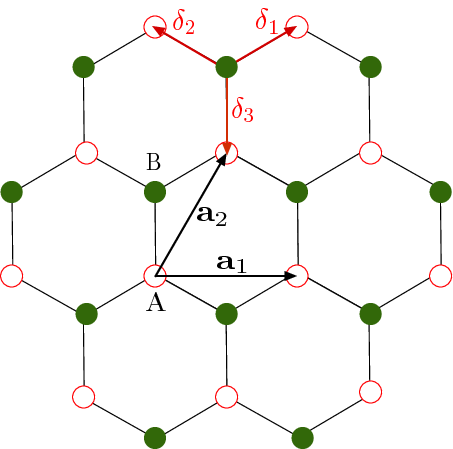
\includegraphics[width=0.5\linewidth]{images/HoneycombGreen}
	\caption{cite http://inspirehep.net/record/1256684/files/HoneycombGreen.png}
	\label{fig:honeycombgreen}
\end{figure}


Where $a_{1,2} =a(\sqrt{3}/2),\pm1/2)$, and $\delta_3 =a(0,-1) $, where a is the lattice spacing as in fig~\ref{fig:honeycombgreen}. Notice there is no A to A and B to B terms, since these 2 can't be different when there is inversion symmetry, and if they are the same the simply add an identity piece to H(k).

If we take the fourier transform now, $c_r = \int_k \frac{dk^2}{(2\pi)^2}e^{-ikr} c_k$, each of the $+\delta$ terms simply contribute an $e^{\pm i k \cdot \delta}$ depending on whether there was a dagger or not. Now we have
\begin{align}
H(k)= 
\begin{pmatrix}
0 & h(k) \\
h^*(k) & 0
\end{pmatrix} \quad h(q) = \sum_i e^{-ik\delta_i} = e^{-ik_ya} + e^{ik_xa\sqrt{3}/2+ik_ya/2}+e^{-ik_xa\sqrt{3}/2+ik_ya/2} \\
h(q) = cos(k_ya)-i sin(k_ya) +(cos(k_ya/2)+i sin(k_ya/2))2cos(k_xa\sqrt{3}/2)
\end{align}
This means that $h_x(k) = cos(k_ya)+2cos(k_xa\sqrt{3}/2)cos(k_ya/2)$ and $h_y(k) = sin(k_ya)-2cos(k_xa\sqrt{3}/2)sin(k_ya/2)$. Notice $h_x(k) = 0$ when $k = \pm K = \frac{2\pi}{3a}(\pm1/\sqrt{3},-1)$, since $h_x(\pm K) = cos(\frac{2\pi}{3})+2cos(\pm\frac{\pi}{3})cos(\frac{\pi}{3})=0$, and $h_y(\pm K) = sin(\frac{2\pi}{3})-2cos(\pm\frac{\pi}{3})sin(\frac{\pi}{3})=0$.

Now that we have this degeneracy, we should talk about the symmetries that protect it. First there is a Time Reversal symmetry T. In general, given any time dependent wave function, the time dependent piece is a bunch of phases $e^{iEt/\hbar}$ onto time independent pieces. Changing the sign of t is equivalent here to complex conjugation, so we will let T be represented by the complex conjugation operator K. Notice that this is dependent on the basis. 
An important point here is that T is anti-unitary. In general under a symmetry S, any correlation function $|<Sa|Sb>| = |<a|b>|$. This means that $|<a|S^TS|b>| =|<a|b>|$ or $|<b|a>|$. Time reversal does the second. There is theorem that says antiunitary symmetries are unitary symmetries with the complex conjugate operator. In our basis, creation and annihilation operators in real space map to real valued matricies, so K leaves them alone. and in k space, sends $c_k$ to $c_{-k}$. We see this if we use the same basis of $\begin{pmatrix}
1 \\
0
\end{pmatrix} = c^{A\dag}_k|0>$ and  $\begin{pmatrix}
0 \\
1
\end{pmatrix} = c^{B\dag}_k|0>$
\begin{align}
THT^{-1}&=\int_{BZ}\frac{dk^2}{(2\pi)^2} 
\begin{pmatrix}
c^{A\dag}_k & c^{B\dag}_k
\end{pmatrix}
TH(k)T^{-1}
\begin{pmatrix}
c^{A}_k \\
c^{B}_k
\end{pmatrix}
 \\
&= \int_{BZ}\frac{dk^2}{(2\pi)^2} 
\begin{pmatrix}
c^{A\dag}_{k} & c^{B\dag}_{k}
\end{pmatrix}
KH(-k)K
\begin{pmatrix}
c^{A}_{k} \\
c^{B}_{k}
\end{pmatrix} = H
\end{align}

This implies $H^*(-k) = H(k)$. In general you can think of a symmetry as both acting on H, and on k.

There is also an inversion symmetry P around the center of a unit cell which sends r to -r. Inversion P sends A sites to B sites, and B to A, while also flipping the sign of k. $\sigma_x$ flips the atoms, so we can let $P=\sigma_x$ in our representation. 

The Inversion operator flips the atoms and r coordinate of our real space c operators. This ends up sending $c^A_k = \int_r e^{-ikr}c^A_r$ to $c^B_{-k}$, and similarly with the rest. Now if we take the same basis as before, this has the effect of making our Hamiltonian
\begin{align}
PHP^{-1}&=\int_{BZ}\frac{dk^2}{(2\pi)^2} 
\begin{pmatrix}
c^{A\dag}_k & c^{B\dag}_k
\end{pmatrix}
PH(k)P^{-1}
\begin{pmatrix}
c^{A}_k \\
c^{B}_k
\end{pmatrix} \\
&= \int_{BZ}\frac{dk^2}{(2\pi)^2}
\begin{pmatrix}
c^{A\dag}_k & c^{B\dag}_k
\end{pmatrix}
\sigma_x H(-k) \sigma_x
\begin{pmatrix}
c^{A}_k \\
c^{B}_k
\end{pmatrix}
= H
\end{align}
Inversion makes sure $\sigma_x H(-k) \sigma_x =H(k)$. 

Together this constrains our hamiltonian. By Time reversal, $Kh_x(k) \sigma_xK = h_x(-k)\sigma_x$, which implies $h_x(-k)=h_x(k)$. Inversion makes $\sigma_x (h_x(k) \sigma_x) \sigma_x =h_x(-k)\sigma_x$ which implies the same thing. This means $h_x(k)$ is even in k. For $h_y(k)$, $K h_y(k) \sigma_y K =-h_y(-k)\sigma_y= h_y(k)\sigma_y$. This implies $h_y(k) = -h_y(-k)$. Inversion this time implies  $\sigma_x h_y(k) \sigma_y \sigma_x =-h_y(-k)\sigma_y=  h_y(k)\sigma_y$, which again is the same thing, making $h_y$ odd under k.

Now the important part, By Time reversal, $Kh_z(k) \sigma_zK = h_z(-k)\sigma_z$, which implies $h_z(-k)=h_z(k)$. Inversion makes $\sigma_x (h_z(k) \sigma_z) \sigma_x = -h_z(-k)\sigma_z$, which implies $-h_z(-k)=h_z(k)$. Now we have $-h_z(-k)=h_z(-k)$, which implies $h_z(k)$ is zero!
This means that when we solve for the spectrum there is no $\sigma_z$ component. Then by squaring the H operator we get
\begin{align}
H^2(k)= \sigma_x^2 h_x^2(k) + \sigma_y^2 h_y^2(k) \\
H^2(k)= h_x^2(k) + h_y^2(k) \\
E(k)=\pm\sqrt{h_x^2(k) + h_y^2(k)}
\end{align}
Now the interesting part here is since we can't add a $\sigma_z$ piece, all we could add is parts to $h_x$ or $h_y$. Since around our K or K' point we have $E(K+q)=\sqrt{q_x^2+q_y^2}$, all we can do is add a constant, which would just shift the dirac points, or add higher order pieces, which still go to zero. Now if we break one of the symmetries we can add $\sigma_z$ pieces, and gap out the system. We will see that there are topologically distinct ways to do this.

If we introduce a small constant $M\sigma_z$ term to H(k), which can be done in real space by adding $Mc^{A\dagger}_rc^A_r - Mc^{B\dagger}_rc^B_r +h.c$ terms to the sum. This breaks our inversion symmetry, and is physically making the atoms on the A site and B site different. In the limit of large M, this is basically binding all the atoms to one site, or a trivial insulator. This was first shown by semenov (cite).

Haldane showed that there is a topologically nontrivial phase here, if you break time reversal but not inversion. The intuition here being if you add a term that is $h_z(k)\sigma_z$ where $h_z(k)=-h_z(-k)$ to preserve time reversal. In the limit that k is close to K
\begin{align}
H(q=(k-K))= \sigma_x h_x(q) + \sigma_y h_y(q) + \sigma_z h_z(q)\\
H(q)= c(\sigma_x q_x + \sigma_y  q_y) + \sigma_z h_z(q)
\end{align}
For some constant c. If $h_z\sigma_z$ is time reversal symmetric, we know what the Hamiltonian will be at near -K as well. 

 He added next nearest neighbor hopping to another 6 sites,such that all lattice symmetries stayed, that added a piece onto H(k) that went as follows.
\begin{align}
H_2(k) =  2t_2 cos(\phi)\sum_i cos(k \cdot b_i)  +2t_2 sin(\phi) \sum_i sin(k \cdot b_i)
\end{align} 
where $b_1 = \delta_2 - \delta_3$, $b_2 = \delta_3 - \delta_1$, and $b_3 = \delta_1-\delta_2.$ This ends up introducing an $h_z(k=\pm K) = \mp 3\sqrt{3}t_2sin(\phi)$. If you think about this in the limit of being close to K or -K, It is the fact that this gap flips sign at $\pm K$ that makes our topology nontrivial.

Our berry curvature integral ends up taking the form
\begin{align}
n = \frac{1}{4\pi}\int_{BZ}dk^2 \partial_{k_x}\hat{h}(k) \times \partial_{k_y}\hat{h}(k) \cdot \hat{h}(k) \\
\hat{h}(k) = \vec{h}(k)/|\vec{h}(k)|
\end{align} 
This just counts the number of times $\hat{h}(k)$ wraps around the unit sphere. Notice this is only defined when there is a gap. In our Semenov/trivial phase, the z component of $\hat{h}(k)$ is always positive. That means $\hat{h}(k)$ can't possibly wrap around the sphere, so n would be 0. In this Haldane phase however, $\hat{h}(\pm K) = (0,0,\mp 1)$, and in fact wraps around the sphere exactly once. This phase actually exhibits a quantum hall conductance of $\sigma_{xy}=e^2/h$. If you put this model on a semi-infinite plane with an edge, you will see a single edge mode which carries this charge. Since this map can't go from n=1 to 0 continuously, the only way to change phases would be to close the gap, i.e. make $\hat{h}(k)$ ill-defined. This is the definition of a topological insulator! 

\subsection{Topological insulators with spin}

Now, this was just a toy model, in real life electrons have spin, and this changes things rather drastically. We follow a model by kane and mele ~\cite{KaneMele}, and written pedagogically in Fradkin's book~\cite{Fradkinbook}. Now we have two copies of the exact same model, one for spin up and one for spin down. We can open up a gap using spin-orbit interactions.

In the haldane model, we looked at the chern invariant which ended up being how many times some vector $\hat{h}(k)$ wrapped around the sphere. Based on the sign difference of that at our old degenerate points we could tell if it wrapped the sphere. The degenerate point $(k_1,k_2)=(\pi,\pi)$, where $k_i$ are reciprocal lattice vectors, was sent to K' under time reversal and inversion. Those relation put constraints on our Hamiltonian. When we involve spin, we can have a new topological invariant, that can be nonzero without time reversal breaking. 

If you talk about spinful electrons, we can take the previous model and double it, one for spin up and one for spin half, and have one be the time reversal copy of the other. Now if the first has a chern number of 1, the second has chern number -1. The total charge conductance cancels out, but there is still a "spin current", since spin ups move say clockwise and spin downs move counterclockwise. The topological invariant associated with this can again be found out by looking at old degenerate points and symmetry constraints.

We now need to find the T operator. An interesting fact here is $T^2 =-1 $ for fermion systems. You can understand this from CPT symmetry. In euclidean space CPT is just a 180 degree rotation. That squared then is a 360 rotation, which is +1 for bosons and -1 for fermions. If we let $(CP)^2=1$ and assume these things commute, then $T^2=-1$. It has to be real valued by the operation we saw above, and has a piece that's $\tau_x$ or $\tau_y$, to switch spins. The $\tau_x$ would give the wrong $T^2$, so we choose $T = i\tau_yK$, and $T^2 = i\tau_yi\tau_yK^2 = i^2 = -1$.

In 2-d spinful systems, there is whats called a kramer's degeneracy protected by just time reversal. If we assume $T|\phi>= e^{i\theta}|\phi>$, meaning $|\phi>$ is an eigenstate of T, then $TT|\phi> = T e^{i\theta}|\phi> = e^{-i\theta}T|\phi>=e^{-i\theta}e^{i\theta}|\phi>= |\phi>$ which implies $T^2=+1$. The contrapositive means if $T^2=-1$ on a state $|\phi>$then $|\phi>$ is not an eigenstate of T. Then if we have time reversal symmetry $T|\phi_1(k)> = |\phi_2(-k)>$ and since H and T commute,
\begin{align}
TH|\phi_1(k)> = TE_1(k)|\phi_1(k)> = E_1(k)|\phi_2(-k)> \\
HT|\phi_1(k)> = H|\phi_2(-k)> = E_2(-k)|\phi_2(-k)> \\
E_1(k)=E_2(-k)
\end{align} 
So if we have a time reversal invariant point, i.e. $k=-k+G$ where G is a reciprocal lattice vector, we have a degeneracy. Again the thing that matters is a different sign on the "mass" at degenerate points. Then the topological invariant is discovered by looking at these degenerate points, or the matrix given by $w_{ij}(k) = <\phi_i(-k)|T|\phi_j(k)>$, This is of interest when k is time reversal invariant. If we assume for a moment that there are only 2 bands, it is nonzero if $i\ne j$. You could guess the sign of the gapping term would be given by the sign of $ \sqrt{\det{w(K)}}$. This is not just a simple $\pm1$, so interestingly enough we use the pfaffian, which remember squares to the determinant. In the 2 x 2 case, it is just $M_{12}$. We define $\delta(k) = \sqrt{\det{w(K)}}/pfaff(w(K)) = \pm 1$, or in the 2 x 2 case = $\pm sgn(w_{12})$ This is interesting because this function is of great importance later in this thesis. One issue is the square root, leaving the sign ambiguous. This is a continuous function however, and you can fix the sign differences at different invariant points is defined. In 2-D there are 4 time reversal invariant momenta $Q_i$, so let $(-1)^\nu = \prod_i \delta(Q_i)$. This thing ends up being gauge invariant and $\nu$ is a topological invariant that carries two values $0,1\mod 2$. It is called time reversal polarization.

This is called a $Z_2$ index. The reason why this is no longer Z classified is that we could have non spin conserving terms that are still time reversal invariant. If you think of N chiral modes on the spin up half, you have N spin down on the bottom. If you try and scatter them, you would have a scattering matrix. If  you have a state
\begin{align}
|\psi_{L}>=\sum_{i=1}^N \alpha_{i,L}|\psi_\uparrow^L>+\beta_{i,L} T|\psi_\uparrow^L> \\
|\psi_{R}>=\sum_{i=1}^N \alpha_{i,R}|\psi_\uparrow^R>+\beta_{i,R} T|\psi_\uparrow^R>  
\end{align}
with $\alpha$'s for the incoming modes and $\beta$'s for the outgoing. The scattering matrix is goes as 

\begin{align}
\begin{pmatrix}
\vec{\beta}_L \\
\vec{\beta}_R
\end{pmatrix}
=
\begin{pmatrix}
r & t\\
t' & r'
\end{pmatrix}
\begin{pmatrix}
\vec{\alpha}_L \\
\vec{\alpha}_R
\end{pmatrix}
\end{align}
Now S has to be unitary since it is a change of basis from incoming to outgoing states. If we act with T on this though, outgoing becomes incoming and ect. S on those now gives $ST^2\vec{\beta}^*=\vec{\alpha}^*$. The reason the $T^2$ is there is because the incoming $\beta$ states previously had no T's and now there are two. If we solve for $vec{\beta}$ we get $\vec{\beta}=T^2S^T\vec{\alpha}$. If $T^2=1$ this means $S=S^T$ together with $S^{-1}=S^\dag$. In this case if we try to let t=t'=0, that just requires r and r' have those same conditions. Yet if $T^2=-1$ that means S is antisymmetric. Then if t=t'=0 that means r and r' are antisymmetric and unitary. But if N is odd, that means we have an odd dimension antisymmetric matrix, which always have a zero eigenvalue which is impossible for a unitary matrix. This means not only that t and t' aren't zero, but that one mode must have perfect transmission. So this topological index simply measures oddness of the number of helical modes.

This generalizes to three dimensions. Then there are 8 invariant points and $(-1)^{\nu_0} = \prod_i \delta_i$, and 3 more invaraints $(-1)^{\nu_k} = \prod_i \delta_i$ where the sum is now just 4 points on the xy, yz, or zx planes of the Brillouin zone. This is just treated the 3d topological insulator as a 2d one in different projections. These three are called weak topological insulators and the sum over 8 is called a strong topological insulator, since it turns out to be robust to disorder.

Here is a brief summary of what we saw in this section. Topological insulators are band insulators that cannot be deformed into the atomic limit insulator without closing the gap. We went through two models of this that exhibit the quantum hall effect and the quantum spin hall effect. The logic is that the symmetries constrain the hamiltonian to have a certain form, and if you start from a semi-metal you can open up a gap in distinct ways. This is tricky as a topological index being zero does not mean the phase is trivial, for instance the quantum spin hall effect has trivial chern number. Even if all the indecies we knew of were zero there might be nonzero ones that we haven't thought of yet. Anyhow a conventional TI has a set of symmetries, so far at minimum time reversal and charge conjugation.
 
This sums up an introduction to tools used in the two papers which I will describe in detail for the rest of this thesis. As a recap, I described classical, integer quantum hall and then fractional quantum hall. Following that we delved into the specifics of a $\nu=1/2$ state. Then we talked about how using conformal field theory, we can analyze excitations here, and describe these states in terms of electronic operators and vice versa, which was part of my groups research. Now we can ask what questions we can answer with this machinery. First, since we can split a dirac mode into Pfaffian modes, we could take all the electrons in a dirac semimetal, and backscatter pfaffian modes to have a new type of gapping. We will explore this first. Next we know the Pfaffian state can live on the surface state of a topological insulator. We could then try to generalize this fractional topological insulators. That is the second publication.
 


